
\section{Key Idea}\label{sec:key-idea}

In a typical naively nested memory layout for arrays of records (Fig.~\ref{fig:memory}) each element in the array is a pointer to a single record object, where each of those objects has a single value for each field of that record.
In the case that these fields are arrays or nested records, they are yet again pointers to that array or record object respectively.
Such a naive nesting requires a large amount of memory allocations, and consequently results in a blowup in the amount of reference counting operations that is required.
Furthermore this naive nesting has a negative impact on the memory locality of these objects;
adjacent record fields in an array of records are no longer adjacent in memory.
This limits the applicability of vectorization of operations on arrays of records.

\begin{figure}[ht!]
    \centering
    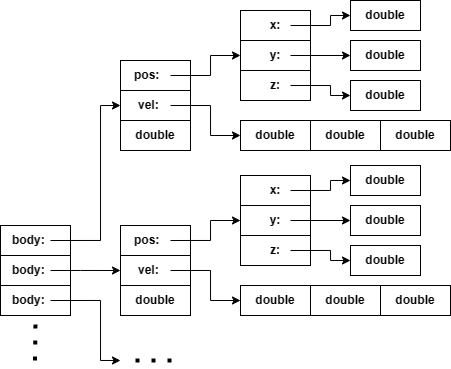
\includegraphics[width=0.7\linewidth]{images/records.png}
    \caption{Naively nested memory layout of the \texttt{Body} record.}
    \label{fig:memory}
\end{figure}

In order to combat these drawbacks we rewrite records into a flattened array representation, where each base-type field is defined by a single array.
Nested records are recursively flattened until only base-types remain.
In the proposed flattened representation, only a single allocation is required for each base-type field of a record.
Consequently this also decreases the amount of reference counting operations that is required, and opens the door to vectorization of operations on these arrays.

This transformation from arrays of records to flattened arrays additionally requires a rewrite of the rest of a program.
Programs need to be rewritten to operate on multiple arrays, instead of on singular arrays of records.
In the case of the n-body example, the record declaration is removed and the acceleration and timestep functions are rewritten to operate on arrays instead.
These functions now require additional arguments and return multiple return values, instead of only a single record.
Unused record fields are removed from these rewritten function definitions. 
Below we show the result of the rewriting process on the acceleration functions from the example.
%
\begin{lstlisting}
double, double, double
acc(double x1, double y1, double z1,
    double x2, double y2, double z2,
    double mass2)
{
    xdir = x2 - x1;
    ydir = y2 - y1;
    zdir = z2 - z1;
    factor = l2norm(xdir, ydir, zdir) == 0.0
        ? 0.0 : m / pow3(l2norm(xdir, ydir, zdir));
    return (xdir * factor, ydir * factor, zdir * factor);
}

double[n], double[n], double[n]
acc_v(double[n] xs, double[n] ys, double[n] zs, double[n] masses)
{
    return { [i] -> rsum(1, { [j] -> acc(xs[i], ys[i], zs[i],
                                         xs[j], ys[j], zs[j],
                                         masses[j])
                            | [j] < [n] })
           | [i] < [n] };
}
\end{lstlisting}
%
The example shows that the transformation is not trivial. 
When arrays and records are combined and nested, the transformation to the required homogeneous arrays by \sac{} can become complex.
To ensure that arrays of records can be transformed into homogeneous arrays we disallow (mutual) recursion and we require that array fields in records are of a statically known and fixed shape.

Additional effort is required for primitive functions, in order for those to be able to operate on record types.
For example, it should be possible to get the dimensionality or shape of an array of records, or to select one of its elements, without the need for a special syntax.
Similarly we need to ensure that tensor comprehensions and other array constructors are able to operate on multiple arguments.
Already in the n-body example we see that often not all fields defined in a record are used by a function, and that not all fields of a record need to be returned.
In order to limit the overhead introduced by an increase in the amount of arguments, and to maximise optimisation potential, two more optimisations are required to remove these unused arguments and return values.



\iffalse
\subsection{Interleaving}

In certain scenarios an interleaved (but flattened) memory layout is actually preferred, as opposed to the suggested flattened notation.
Consider the position field from the body record.

\begin{lstlisting}
struct Body {
    double[3] pos;
    double[3] vel;
    double mass;
}
\end{lstlisting}

Given a vector of these bodies, the positions will become an \texttt{[n,3]} array where the x-y-z coordinates of each position follow each other in memory.
However in the case where we want to apply an operation on only the x-coordinates of a vector of bodies, such a memory layout is not beneficial as the y and z coordinates avoid these operations from being vectorized.
This however can be resolved by expressing the record differently.
Instead of having the position be a three-element vector, it can be represented as a record:

\begin{lstlisting}
struct Pos {
    double x;
    double y;
    double z;
}
\end{lstlisting}

With this notation each coordinate will be expanded into a separate array, now allowing for vectorization of these operations on only the x-coordinates of these bodies.
This example highlights how one can play with the combination of arrays and records in order to obtain the most efficient memory layout.
\fi
